\begin{frame}
\frametitle{Sensitivity Analysis}
Dakota was wrapped around Cyclus to randomly sample various parameters for critical sub-processes:
\begin{itemize}
	\item Electrorefiner
	\item Electrowinner
\end{itemize}

\begin{figure}
	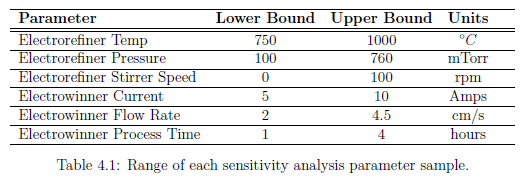
\includegraphics[width=\linewidth]{sens-params}
\end{figure}
\end{frame}

\begin{frame}
\frametitle{Electrorefiner - Temperature}
\begin{figure}
	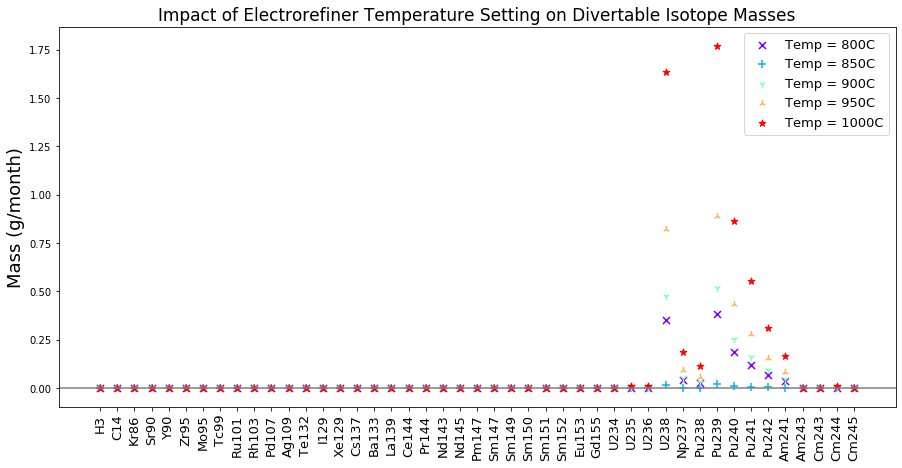
\includegraphics[width=\linewidth]{./images/temperature-sa-diff}
\end{figure}
\end{frame}

\begin{frame}
	\frametitle{Electrorefiner - Stirrer}
	\begin{figure}
		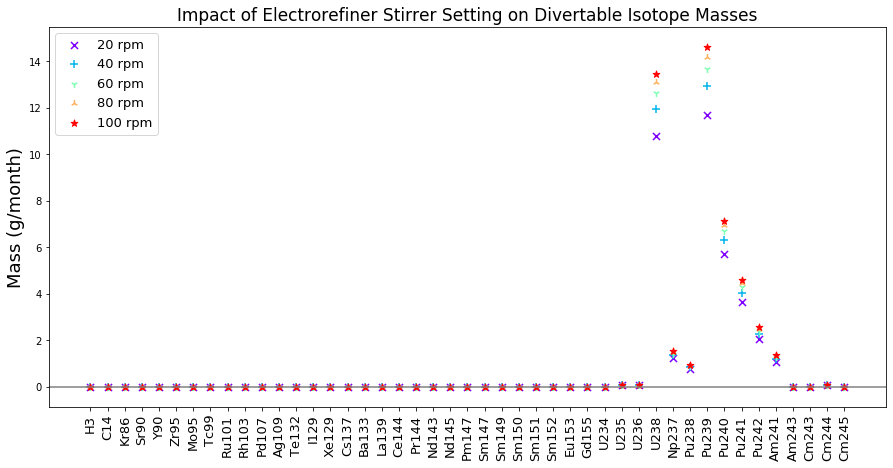
\includegraphics[width=\linewidth]{./images/rotation-sa-diff}
	\end{figure}
\end{frame}

\begin{frame}
	\frametitle{Electrowinner - Current}
	\begin{figure}
		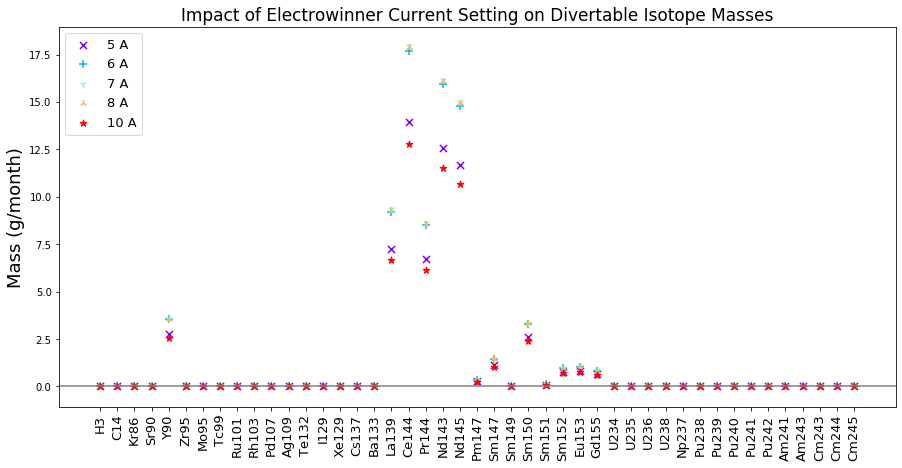
\includegraphics[width=\linewidth]{./images/current-sa-diff}
	\end{figure}
\end{frame}

\begin{frame}
	\frametitle{Electrorefiner - Process Time}
	\begin{figure}
		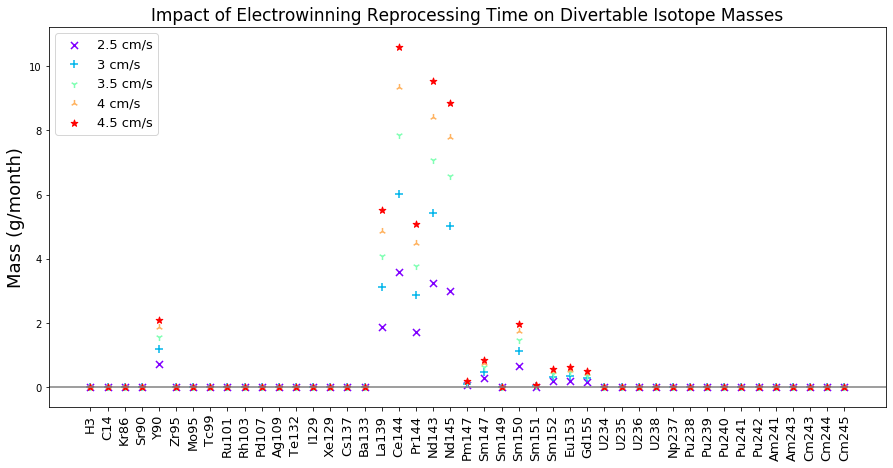
\includegraphics[width=\linewidth]{./images/time-sa-diff}
	\end{figure}
\end{frame}

\begin{frame}
\frametitle{Sensitivity Results}
	Parameters that influenced interaction between eutectic and waste showed more significant impact on separation efficiency.
	\begin{figure}
		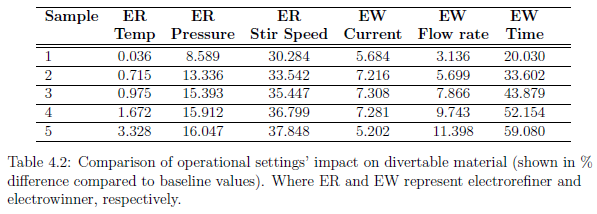
\includegraphics[width=\linewidth]{sens-results}
	\end{figure}
\end{frame}